\subsection{Single Transistor Circuits}
MOSFETS are cool. They really have multiple modes of function with their different "regimes", which allow them to preform several functions. One thing to keep in mind before starting to look at circuits is that, as a rule of thumb, circuits are always drawn in a way to have the higher potential on top and the lowest potential on the bottom of the circuit. So you'll pretty much always see ground at the bottom and $V_{dd}$ at the top, hopefully this will help you read through the circuits more easily. 


\subsubsection{The Current Source}
The simplest function of a MOSFET, it is obtained by holding source, drain and gate voltage at constant values. As long as the difference between the drain and source voltages is larger than approximately $4U_T$, and that $V_{gs} < 0.7V$ the nFET in \textbf{saturation and subthreshold} reduces to:

\begin{equation}
    I_{ds} =  I_{n0} e^{\frac{\kappa_{n}V_g - V_s}{U_T}} 
\end{equation}

Remember from our previous discussion of second order effects (see section \ref{subsection:second_order_effects} that this is a First-Order approximation (i.e., it neglects Second-Order effects such as the Early Effect). This basically yields the assumption that the drain current is independent of the drain voltage in Saturation. Note that most often, current source encountered in circuits are pFETs rather than nFETs.

\begin{figure}[H]
    \centering
    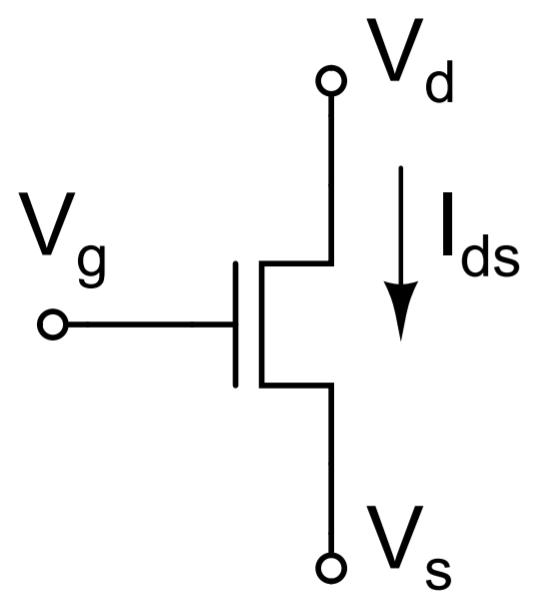
\includegraphics[width=0.25\linewidth]{../../Figures/N_FET_Current_Source.PNG}
    \caption{nFET Current Source. Adapted from Lecture Notes.}
    \label{fig:basalandcerebellum}
\end{figure}

\subsubsection{Linear Resistor}

With some calculation and a lot of approximation, we can reach Ohm's relation, back from the known $I_{ds}$ equation. This means we have a value that links between voltage and current: resistance. Let's start with the subthreshlold equation, but without assuming saturation: 

\begin{equation}
I_{ds} = I_{n0} e^{\frac{\kappa_{n}V_g}{U_T}}(e^\frac{-V_s}{U_T} - e^\frac{-V_d}{U_T}) 
\end{equation}
With some rearranging, we get: 
\begin{equation}
I_{ds} = I_{n0} e^{(\frac{\kappa_n V_g}{U_T}-\frac{V_d + V_s}{2U_T})}(e^{\frac{V_d - V_s}{2U_T}} - e^{-\frac{-(V_d - V_s)}{2U_T}})
\end{equation}
Lucky us, the second term looks like a sinh! (As $sinh(x) = \frac{e^x - e^{-x}}{2}$). 
We thus reach: 
\begin{equation}
I_{ds} = 2I_{n0} e^{(\frac{\kappa_n V_g}{U_T}-\frac{V_d + V_s}{2U_T})}sinh(\frac{V_d - V_s}{2U_T})
\end{equation}
And here comes the approximation that will please mathematicians: If $V_d - V_s$ is small enough (i.e., if we are in the ohmic region), we can approximate the sinh with Taylor Series while neglecting higher order effects: 
\begin{equation}
I_{ds} \approx  I_{n0} e^{(\frac{\kappa_n V_g}{U_T}-\frac{V_d + V_s}{2U_T})}\frac{V_d - V_s}{U_T}
\end{equation}

Now if we freeze $V_d$, $V_s$ and $V_g$, our MOSFET suddenly starts acting like a linear resistor with the following relation: 

\begin{equation}
R = \frac{U_T}{I_{n0}}e^{\frac{V_d + V_s}{2U_T} - \kappa_n \frac{V_g}{U_T}}
\end{equation}

I think it's really sad that I took the time to write all these equations and we don't even need to know them by heart. I hope my suffering got you to at least understand the gist of what using a transistor as a resistor is about. Though there remains an important question: 

\textbf{Why should we bother implementing a resistor with a Transistor instead of just using an actual resistor?}

Good question, and I'm glad you asked. Well in standard CMOS circuits, you're dealing with very very small material, and resistors of this size are very unpractical. It also makes it a lot easier for building purposes, as you don't need to add another type of components to the circuit - Transistor can do everything you need! Another important advantage is that we can change the value of the resistance of the transistor, whereas it is fixed with a physical resistor. Though in most cases, we use a Transconductance amplifier to implement a resistance, but more on this in a dedicated chapter!

\subsubsection{Non Linear Current-Voltage / Voltage-Current Converter}

Sometimes you really need a Gin-Tonic, but all you have at home for you and your friends is juice. Conversely, sometimes you really need a nice juice to forget your difficult night out of the day before, but all you have is Gin left-overs. It would be so convenient if you could easily turn one into the other? It's the same in electrical circuits, where you sometimes need voltage for a given operation, but all you have to give is current, or the opposite. Well, with Transistors, you can convert a current into a voltage, and vice versa! 
Remember from \ref{eq:subsatcurrent} that MOSFET operating in saturation and subthreshold can generate a drain current which is an \emph{exponential} function of $V_{gs}$. Now if you take a current as the input signal, we can isolate $V_g$ or $V_s$ and make it the output signal. This was a bit counter intuitive to me at first: we've always looked at voltages as the first thing to apply to obtain current. But it does make sense that if you \emph{force} a current into a transistor, the voltage will have to follow in order to satisfy their expected behaviour. In subthreshold, we can re arrange \ref{eq:subsatcurrent} and isolate $V_s$ or $V_g$ as follows:  

\begin{equation}
V_s = \kappa_n V_g - U_T log(\frac{I}{I_{n0}}),
\end{equation}
\begin{equation}
V_g = \kappa_n^{-1}(Vs + U_T log(\frac{I}{I_{n0}})
\end{equation}

\subsubsection{Diode Connected Transistors}

This one can be tricky at first, and it's very important to understand it properly. 

\begin{figure}[H]
    \centering
    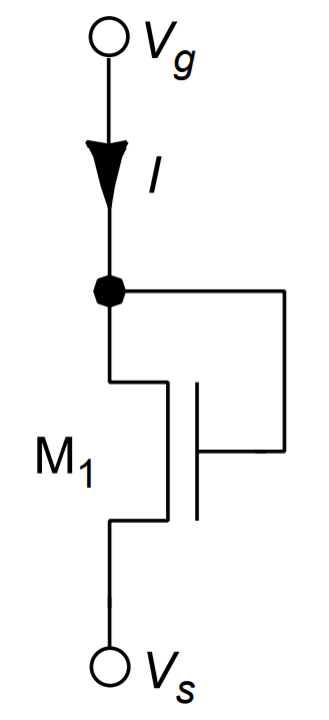
\includegraphics[width=0.15\linewidth]{../../Figures/Diode_Connected_NFET.PNG}
    \caption{Diode Connected nFET. Adapted from Lecture Notes.}
    \label{fig:diode_connected}
\end{figure}


In this circuit, we connect the gate to the drain: $V_g = V_d$. This reduces the transistor to a two terminal device, similar to a diode, hence its name diode connected. Understanding the property of the circuit is actually simpler with the help of the equations than words. If we go from our full subthreshold equation \ref{eq:fullsubcurrent}:

\begin{equation}
I_{ds} = I_{n0} e^{\frac{\kappa_{n}V_g}{U_T}}(e^\frac{-V_s}{U_T} - e^\frac{-V_d}{U_T})
\end{equation} 

we can rearrange as follows by replacing $V_d$ with $V_g$: 

\begin{equation}
I_{ds} = I_{n0} e^{\frac{\kappa_{n}V_g}{U_T}}(e^\frac{-V_s}{U_T} - e^\frac{-V_g}{U_T}) = I_{n0} (e^{\frac{\kappa_{n}V_g - V_s}{U_T}} - e^\frac{\kappa_{n}V_g - V_g}{U_T})
\end{equation}

\begin{equation}
I_{ds} = I_{n0} e^{\frac{\kappa_{n}V_g - V_s}{U_T}} - e^\frac{\kappa_{n}V_g - V_g}{U_T}
\end{equation}

Remember, we love assumptions and simplifications of calculations here. So we keep on assuming that $\kappa_n \approx 1$ 

\begin{equation}
    I_{ds} \approx I_{n0} e^{\frac{\kappa_{n}V_g - V_s}{U_T}} - e^\frac{V_g- V_g}{U_T}
\end{equation}

and thus reach back the familiar saturation equation:

\begin{equation}
I_{ds} \approx I_{n0} e^{\frac{\kappa_{n}V_g - V_s}{U_T}}
\end{equation}

So now, when a transistor is diode connected, it actually \emph{necessarily operates in saturation}, it's not an assumption anymore (well it always kinda is, but less than before :) ). Now the critical thing to understand is that the first thing happening here is current flowing into a transistor (just imagine a current source as described before). The current flowing creates a feedback loop between the drain and the charge where both automatically adapt to match each other and work saturation. So the current is what sets the gate voltage! This is very important as it is a clever way to adjust gate voltage from the current, which is typically not possible as there is infinite impedance between the channel (source, drain and well) and the gate. 